\documentclass[a4paper,11pt]{article}

\usepackage{graphicx}
\usepackage{amsmath}
\usepackage{blindtext}
\usepackage{apacite}
\usepackage{tabularx}
\usepackage{multirow}
\usepackage{geometry}
	\geometry{
	margin = 1in
}
\usepackage{pdflscape}
\usepackage{fancyhdr}
	\pagestyle{fancy}
	\lhead{}
	\chead{}
	\rhead{}
	\lfoot{}
	\cfoot{}
	\rfoot{\thepage}
	\renewcommand{\headrulewidth}{0pt}
\usepackage[T1]{fontenc}
\usepackage[math]{iwona}
\usepackage{mathptmx}
\usepackage{longtable}
\usepackage{caption}
	\setlength{\abovecaptionskip}{0.5em}
\usepackage{makecell}

\title{\Huge{ENG2016: Bike Project}}
\author{\begin{tabular}{l c}
		Ivan Mihajlovic&2239242 \\
		William Ely&2292204 \\
		Qiyu Zhang&2295435 \\
		Ewan Walker&2235937 \\
		Eduard Fiedler&2248902 \\
\end{tabular}
}
\date{2018}

\linespread{1.25}

\renewcommand{\contentsname}{Table of Contents}

\begin{document}

\pagenumbering{roman}

\begin{titlepage}

	\vspace*{\fill}
    	\begin{center}
		\LARGE{\textsc{University of Glasgow}}\vspace{2em} \\

		\hrulefill\\
		\vspace{0.8em} 
		\Huge{ENG2016: Bike Project}\\\hrulefill
		\vspace{2em}\\
		\LARGE{
			\textsc{Group 23}\vspace{2em}\\
			\begin{tabular}{l c}
				Ivan Mihajlovic\phantom{W}&2239242 \\
				William Ely&2292204 \\
				Qiyu Zhang&2295435 \\
				Ewan Walker&2235937 \\
				Eduard Fiedler&2248902 \\
			\end{tabular}}\\
    	\end{center}
    	\vspace*{\fill}
	\vspace{10em} 

\end{titlepage}

\setcounter{page}{2}

\section*{Abstract}
\addcontentsline{toc}{section}{Abstract}

The purpose of this project is to design an electric bicycle for 55+-year-old men. The goal is to provide insight on the thought process and decision making behind the final design, and how it will be implemented into the current market. This has been done by examining the growing market of electric bikes, and applying sufficient research, in order to construct a realistic bicycle. After analysing multiple different concepts, it was concluded that a men�s Dutch style bike was the ideal design as it allowed a stylish, and comfortable means of commute, in comparison to alternatives.

\pagebreak

\tableofcontents

\pagebreak

\listoftables
\addcontentsline{toc}{section}{List of Tables}

\pagebreak

\listoffigures
\addcontentsline{toc}{section}{List of Figures}

\pagebreak

\pagenumbering{arabic}

\section{Introduction}

With a growing interest in battery powered transportation devices, the electric bicycle has experienced a worldwide, rapid growth in popularity since 1998 \cite{wein07}. However, many companies try to sell their product as an athletic alternative, this caters towards young to middle-aged adults (20-40 years old), and neglects the older population. 

The aim is to design an e-bike that accommodates an older audience by reducing effort, emphasising ergonomics, and improving the quality of their commute. The final product is targeted towards a male market, above the age of 55, and will provide these characteristics in an exceptional manner.

This report will convey the emulation of a typical design process, the means used to conduct decisions for the final design, and its implementation into the current market.

\section{Project Planning}

In order to remain organised, a Gantt chart was formulated. The Gantt chart allowed a visualisation of work allocations for the various topics that were required to complete the project. 

\subsection{Initial Work Allocations}

\begin{table}[!ht]
	\centering
	\caption{Initial Gantt chart}
	\begin{tabular}{l || c  c  c  c  c  c  c  c  c  c  c }
		\multicolumn{1}{l||}{Task}&W1&W2&W3&W4&W5&W6&W7&W8&W9&W10&W11\\\hline\hline
		Research&&&\multicolumn{1}{|c|}{\footnotesize{ALL}}&&&&&&&&\\ \hline
		PDS&&&\multicolumn{2}{|c|}{\footnotesize{ALL}}&&&&&&&\\\hline
		Concept Generation&&&&\multicolumn{2}{|c|}{\footnotesize{ALL}}&&&&&&\\\hline
		CAD&&&&&\multicolumn{3}{|c}{\footnotesize{EW-ED-IV}}&\multicolumn{1}{|c}{\phantom{.}}&&&\\\hline
		Market Analysis&&&&&\multicolumn{2}{|c|}{\footnotesize{QIYU}}&&&&&\\\hline
		House of Quality&&&&&&\multicolumn{2}{|c}{\footnotesize{WILLIAM}}&\multicolumn{1}{|c}{\phantom{.}}&&&\\\hline
		Report&&&&&&&&\multicolumn{4}{|c}{\footnotesize{ALL}}\\\hline
		Presentation&&&&&&&&\multicolumn{4}{|c}{\footnotesize{ALL}}\\\hline
		Group Meetings&&\multicolumn{10}{|c}{\footnotesize{ALL}}
	\end{tabular}
\end{table}

In terms of initial work distribution, the complexity of each topic was allocated between the group members based on: background, and abilities. This required the distribution of the CAD work amongst 3 people, as it was speculated to take longer. Furthermore, in the initial stages group work was emphasised to integrate individual concepts, and weekly meetings were scheduled in order to remain on the same page.

\subsection{Final Work Allocations}

As progress was made with the project, initial roles couldn't be maintained due to different individual schedules. Additionally, by further expanding on the generalised topics in the previous chart, the work had to be allocated differently. This resulted in the following work distribution in order to complete the project on time.

\begin{table}[!ht]
	\centering
	\caption{Final Gantt chart}
	\begin{tabular}{ l || c  c  c  c  c  c  c  c  c  c  c }
		\multicolumn{1}{l||}{Task}&W1&W2&W3&W4&W5&W6&W7&W8&W9&W10&W11\\\hline\hline
		PDS&&&\multicolumn{3}{|c|}{\footnotesize{ALL}}&&&&&&\\\hline
		Concept Designs&&&\multicolumn{2}{|c}{\footnotesize{ALL}}&\multicolumn{1}{|c}{\phantom{.}}&&&&&\\\hline
		Biomechanics&&&&&\multicolumn{5}{|c|}{\footnotesize{QI}}&\\\hline
		Market Analysis&&&&&\multicolumn{5}{|c|}{\footnotesize{WILLIAM}}&\\\hline
		House of Quality&&&&&\multicolumn{5}{|c|}{\footnotesize{EDUARD}}&\\\hline
		Detailed Sketches&&&&&\multicolumn{3}{|c|}{\footnotesize{ALL}}&&&\\\hline
		Components&&&&&\multicolumn{1}{|c}{\footnotesize{ALL}}&\multicolumn{4}{|c|}{\footnotesize{IVAN}}&\\\hline
		Materials&&&&&&\multicolumn{4}{|c|}{\footnotesize{IVAN}}&\\\hline
		Design Analysis&&&&&&&\multicolumn{2}{|c|}{\footnotesize{ALL}}&&&\\\hline
		CAD&&&&&\multicolumn{5}{|c|}{\footnotesize{EWAN}}&\\\hline
		Costing&&&&&&&\multicolumn{3}{|c|}{\footnotesize{IVAN}}&&\\\hline
		Group Meetings&&\multicolumn{10}{|c}{\footnotesize{ALL}}\\\hline
		Presentation&&&&&&&&\multicolumn{4}{|c}{\footnotesize{ALL}}\\\hline
		Report&&&&&&&&\multicolumn{4}{|c}{\footnotesize{ALL}}\\\hline
		Evaluation&&&&&&&&&&&\multicolumn{1}{|c}{\footnotesize{ALL}}
	\end{tabular}
\end{table}

\section{User Requirements}

\subsection{Identifying the Target Market}

\begin{itemize}
	\setlength{\itemsep}{0pt}
	\item Designed for a 55+ year old man who is commuting to work in the city
	\item Design should be comfortable and accommodate non-conventional riding gear such as a full suit
	\item Expected to be transporting at least one piece of luggage, e.g. briefcase
	\item Wants to arrive to work without being sweaty
	\item Relatively fit, travelling a maximum of 50km per day (to and from work)
	\item Tenured employee with sufficient funds
\end{itemize}

\subsection{Product Design Specification}

\begin{longtable}{l l c}
	\hline
	Category&Specification&Importance (1-5)\\\hline
	\makecell[l]{Technical Requirements\\ \\}&\makecell[l]{Despite being electrically assisted, operation for \\the user should resemble that of a normal push bike}&\makecell[c]{3}\\ \cline{2-3}
						 &\makecell[l]{According to EU regulations, the motor will assist\\up to maximum speeds of 25 km/h}&\makecell[c]{5}\\ \cline{2-3}
						 &\makecell[l]{The bike's structural integrity should withstand worst\\case loading scenarios without permanent\\deformations}&\makecell[c]{5}\\ \cline{2-3}
						 &\makecell[l]{Mechanical components should withstand at least\\20,000 operational hours}&\makecell[c]{4}\\ \cline{2-3}
						 &\makecell[l]{The frame should withstand the weight of a\\55-year-old man up to the 95\textsuperscript{th} percentile $\approx$ 113kg}&\makecell[c]{4}\\ \cline{2-3}
						 &\makecell[l]{Wheels, rims, gearing, and turning angles should be\\optimised for a city environment}&\makecell[c]{3}\\ \cline{2-3}
						 &\makecell[l]{According to EU regulations, maximum motor power\\of 250W.}&\makecell[c]{5}\\ \cline{2-3}
						 &\makecell[l]{Components should not be compromised structurally\\and accommodate for thermal expansion between -30\\to 60$^{\circ}$C}&\makecell[c]{2}\\ \cline{2-3}
						 &\makecell[l]{Design should accommodate a solution for\\comfortably transporting at least one suitcase.}&\makecell[c]{4}\\ \cline{2-3}
						 &\makecell[l]{Full-cycle recharging of the battery should be within\\4 hours}&\makecell[c]{3}\\ \cline{2-3}
						 &\makecell[l]{Battery should offer a minimum range of 70km} &4\\ \hline
	Ergonomics&Design should offer a comfortable riding position&4\\ \cline{2-3}
		  &\makecell[l]{Emphasis on comfort should be placed on points of\\contact such as the handlebars and the seat.}&\makecell[c]{3}\\ \cline{2-3}
		  &\makecell[l]{Bike geometry should not stress common points of\\injury such as lower/upper back, neck, and knees.}&\makecell[c]{3}\\ \cline{2-3}
		  &\makecell[l]{A  non-trained person could assemble/disassemble the\\bike within 60 minutes.}&\makecell[c]{2}\\ \cline{2-3}
		  &\makecell[l]{Feet should not slide off the pedals during\\normal operation.}&\makecell[c]{3}\\ \cline{2-3}
		  &\makecell[l]{Battery should be rechargeable from a conventional\\outlet, such as the ones found at home or work.}&\makecell[c]{5}\\ \cline{2-3}
		  &\makecell[l]{Bike should offer different driving modes such as\\disengaging the motor and economy mode.}&\makecell[c]{3}\\ \hline 
	\makecell[l]{Maintenance\\ \\}&\makecell[l]{Battery should not require changing or maintenance\\for at least 1,000 charging cycles.}&\makecell[c]{3}\\ \cline{2-3}
				      &\makecell[l]{Mechanical components which are non-specific for\\the bike design should be readily available}&\makecell[c]{4}\\ \cline{2-3}
				      &\makecell[l]{Motor should be reliable, and in case of failure it\\should be serviced by an expert mechanic}&\makecell[c]{4}\\ \cline{2-3}
				      &\makecell[l]{Sensors and tools available on-board of bicycle, \\should offer the user information about possible\\system failures}&\makecell[c]{3}\\ \cline{2-3}
				      &\makecell[l]{Battery should be easily accessible whilst being\\shielded from the environment}&\makecell[c]{3}\\ \cline{2-3}
				      &\makecell[l]{To avoid mechanical component degradation, mild\\corrosion resistance should be provided for water,\\salt, dust, wind, ice, rocks, oil, and gasoline.}&\makecell[c]{3}\\ \cline{2-3}
		   &\makecell[l]{Suspension should not only provide comfort for the\\user, but also protect the electrical hardware.}&\makecell[c]{4}\\ \hline
	\makecell[l]{Safety\\ \\}&\makecell[l]{A full stop from 25 km/h should be achieved within\\a braking distance of 8 m.}&\makecell[c]{4}\\ \cline{2-3}
				 &\makecell[l]{Chain should be protected from the driver's attire\\and environment}&\makecell[c]{3}\\ \cline{2-3}
				 &\makecell[l]{Street accessories as per law, such as alights,\\reflectors, and brakes.}&\makecell[c]{5}\\ \cline{2-3}
				 &\makecell[l]{Battery should be compatible with different outlets\\and standards to avoid failure during charging.}&\makecell[c]{5}\\ \cline{2-3}
				 &\makecell[l]{Control system should include a feedback loop to\\avoid exposing components to voltages and currents\\outside operational ranges.}&\makecell[c]{5}\\ \cline{2-3}
	      &\makecell[l]{The explosion from a punctured tyre should be\\minimised.}&\makecell[c]{4}\\ \hline
	\makecell[l]{Cost\\ \\ \\}&\makecell[l]{Final product price should be a bit higher than\\the market average, within the range of \textsterling 1,500 -\\\textsterling 2,200}&\makecell[c]{4}\\ \cline{2-3}
				  &\makecell[l]{Self-maintenance cost should be similar to that\\of a conventional push bike.}&\makecell[c]{3}\\ \cline{2-3}
				  &\makecell[l]{Battery replacement should be within the range of\\ \textsterling 200 - \textsterling 300.}&\makecell[c]{3}\\ \cline{2-3}
				  &\makecell[l]{Average market price (disregarding economies\\of scale) should be taken for individual components\\and materials for the cost report}&\makecell[c]{3}\\ \cline{2-3}
				  &\makecell[l]{The bike should be a long-term investment with an\\ensured ROI when compared to conventional\\transport methods offered within the city (incentive\\for potential customers)}&\makecell[c]{5}
\end{longtable}

\section{Biomechanics}

\section{Current Market Analysis}

\section{Conceptual Design}

\subsection{Initial Sketches}

\subsection{Morphological Analysis}

\section{Quality Function Deployment}

In order to meet customer demands, research and initial product specifications are combined to form the House of Quality. The aim is to produce a customer driven product which will fulfil key demands, by translating user requirements into engineering requirements. Then, by comparing the individual aspects, the importance can be visualised and securely compromised if they are deemed unimportant to the design.

\subsection{Engineering Specifications}

\begin{table}[!ht]
	\centering
	\caption{Translation of user requirements}
	\begin{tabular}{l l l}
		\hline
		Category&User Requirements&Engineering Specifications\\\hline
	Performance&Bike parts will last for a long time&Fatigue Limit Cycles\\
		&Adequate gearing for a city environment&Number of Gears\\
		&Mobility at moderate speeds&Turning radius at 20km/h\\
		&Temperature resistant&Melting point of Material\\
		&Corrosion resistant&Based on material selection\\
		&Luggage space&Amount of suitcases supported\\
		&High acceleration from rest&Effort required for acceleration\\
		&Low-effort for commute&Effort required for distance\\
		&Supports the weight of the rider&Material yield strength\\
		&Good braking&Braking distance from max speed\\
		&Low centre of gravity&Height of C.o.G. above ground\\\hline
	Battery&High battery capacity/battery lifespan&Battery capacity\\
		&Battery assists up to specified speed&Input choked at certain speed\\
		&Battery recharges quickly&Recharge cycle time (full)\\
		&Battery supports significant power&Work input\\\hline
	Suspension&No deformations due to vibrations&Material yield strength\\
		&Remains steady at high speeds&Structural vibrations\\
		&Smooth ride&Spring stiffness\\\hline
	Ergonomics&Comfortable riding position&Amount of satisfied people\\
		&Height adjustable seat and handlebars&Range of adjustment\\
		&Easy to assemble&Assembly time\\
		&Easy to maintain&Amount of tools required\\
		&Easy to carry&Overall weight of bicycle\\
	\end{tabular}
\end{table}

When translating user requirements to engineering specifications, various methods of testing and measuring are used to describe them. In terms of performance, properties of the general structure of the bike, and its functionality are considered. Furthermore for the battery and the suspension, these characteristics were considered outside of the performance, as they are aspects that must be well defined for the end design of the bike. Lastly, requirements categorised as ergonomics, are quantified in terms of ease of use and comfort.

\subsection{Analysis}

To form the House of Quality, the following investigations were made to find relationships between the requirements:
\begin{itemize}
	\setlength{\itemsep}{0pt}
	\item What vs. How? (User requirements vs. Engineering specifications)
	\item How vs. How? (Engineering specifications vs. Engineering specifications)
	\item Who vs. What? (Potential buyers vs. User requirements)
	\item Now vs. What? (Similar products on the market vs. User requirements)
	\item How much? (What are the feasible targets in terms of engineering specifications)
\end{itemize}

In the first phase of analysis, User requirements and Engineering specifications are inspected for relationships (middle area of table~\ref{tab:hoq}). First, each engineering specification was identified with its corresponding unit of measurement and the direction in which it should be improved. Furthermore, from the colours it is apparent that the diagonal line of strong relationship is due to each user requirement having its own engineering specification. From this the main points of focus became:
\begin{itemize}
	\setlength{\itemsep}{0pt}
	\item High battery quality which has properties that compliment each other and will demonstrate performance
	\item The weight of the bicycle will have a large impact on all other requirements which means that it must be reduced as much as possible
	\item Suspension, overall comfort, and battery power will be able to reduce the effort of the rider which pairs with the main objective
\end{itemize}

Next, engineering specifications are evaluated for potential relationships (roof). This analysis further reveals the importance of reducing the weight, and further confirms how effort of the rider will be minimised. The latter requirement primarily requests for sufficient battery quality, which needs to be implemented into the final design. Lastly in terms of suspension, the safety of the rider will essentially be improved, by protecting the bike during operation and potentially reducing braking distances.

Potential buyers are then considered and scored based on how important they find the functional (user) requirements (left columns of table~\ref{tab:hoq}). In this case, 3 potential buyers are considered, and how they would potentially rank the importance of the selected requirements. The numbers sum up to 100, which means that an average importance lies at around 4. The following describes how the scores were evaluated:
\begin{itemize}
	\setlength{\itemsep}{0pt}
	\item The target commuter will value high performance, battery quality, and comfort
	\item The recreational user will value battery quality, and ergonomics
	\item The retailer/sales person will require a balance bike, with good adjustability to market to his customers
\end{itemize}

In order to visualise where the final product would rank within the current market, competitors are scored based on how well they fulfil the same user requirements (right column of table~\ref{tab:hoq}). Here, a low-end bicycle (Greenedge CS2), and a high-end bicycle (Trek Lift+ Men) are qualitatively judged, where 5 is excellent, and a 1 is poor. Since the bikes considered tend to a similar market, the rankings are based on customer reviews and individual specifications. Since the selected design is supposed to fill the price range between the two (see PDS), its ranking is also kept between them. Slight improvements in terms of luggage, centre of gravity, and ride quality over the high-end bicycle are desired in order to better fulfil the main objective.

Taking the existing information of the competitors into account, the targets for the design can be specified in the bottom rows of table~\ref{tab:hoq}.

\newpage

\newgeometry{margin=1cm}
\thispagestyle{empty}
\begin{landscape}

\begin{table}[ht]
	\centering
	\caption{House of Quality}
	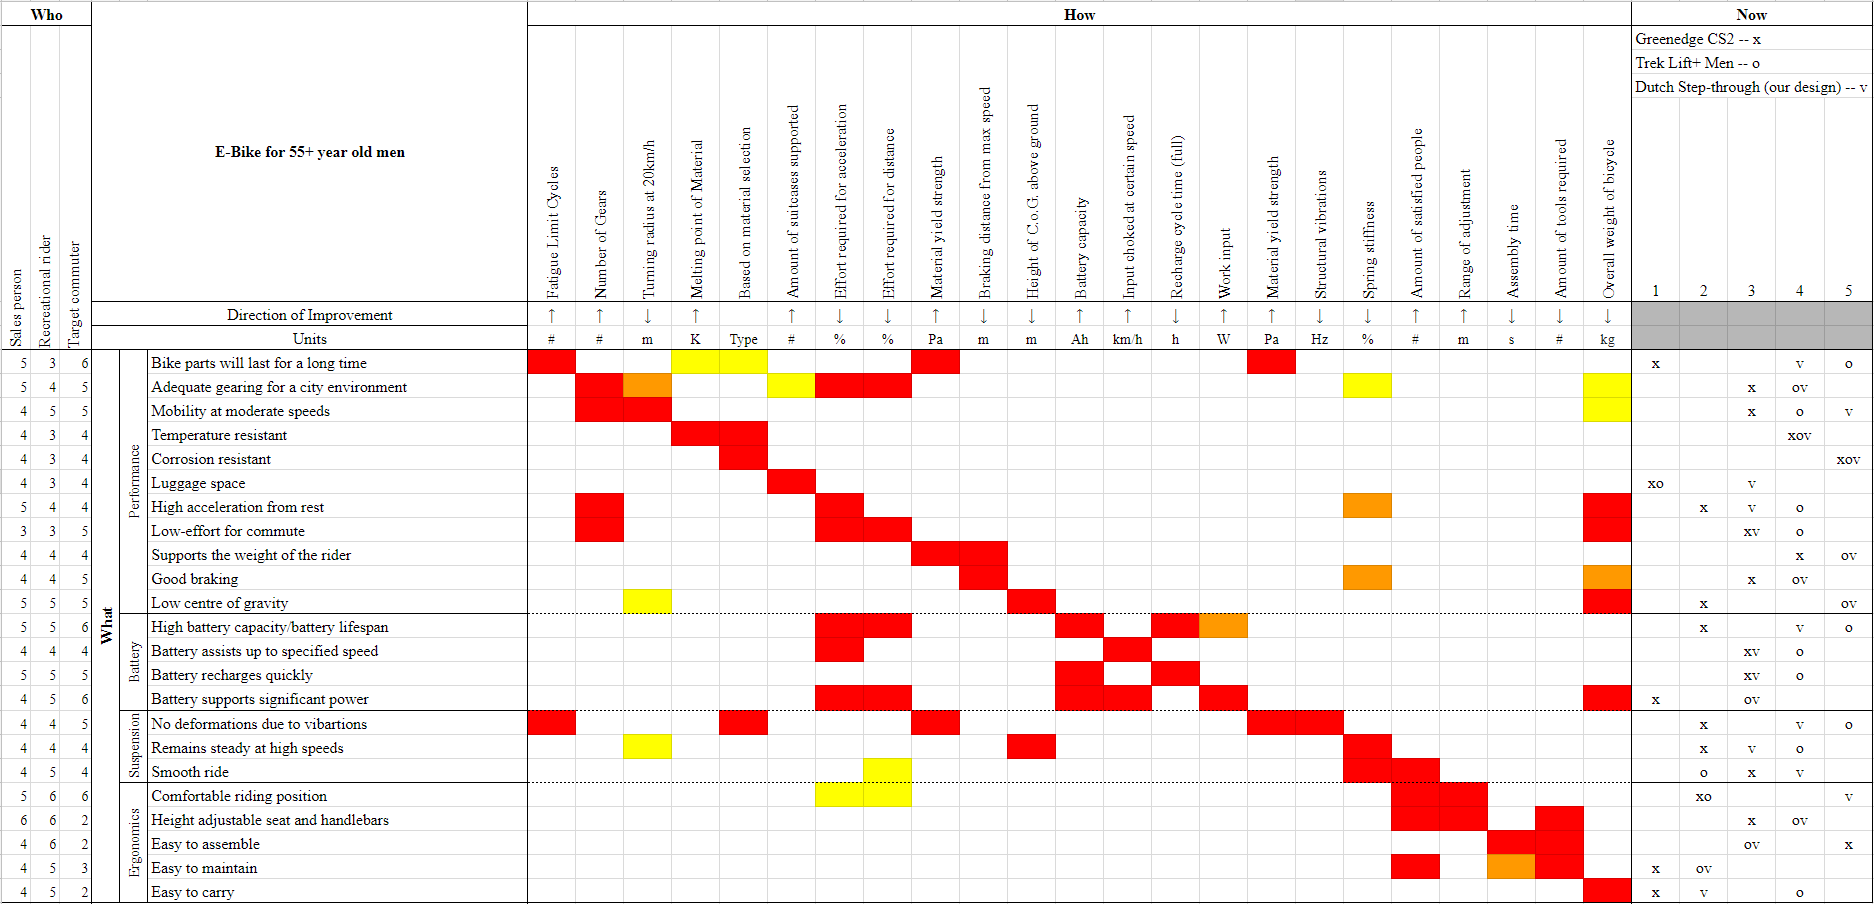
\includegraphics[width=1.45\textwidth]{Hoq}
	\label{tab:hoq}
\end{table}

\end{landscape}
\restoregeometry

\section{Detailed Design}

\subsection{Components}

\subsection{Material Selection}

\subsection{Calculations}

\subsection{Standards Considered}

\section{Costing and Implementation}

The intended product price from the Product Design Specification is between \textsterling1,700 and \textsterling2,200. This price range was selected to be competitive in the e-bike market, by being placed slightly over the average price. Additionally, it is expected that the designed e-bike would not have much competition due to this being an undeveloped market; classic e-bikes as opposed to sport e-bikes. 

The calculations are based on an assumption, where a new product is being developed for a large company. Therefore, the overheads will not be considered as the bike will be one of their many products. Furthermore, all the hardware and software have already been purchased. 

\[
	\text{Selling Price} = \text{Profit} + \left(\text{Works Cost Price} + \left(\frac{\text{Cost of Design}}{\text{Quantity}}\right)\right)
\]

\subsection{Cost of Design}

The cost of design describes the price which is invested into each bicycle. This includes the design labour (i.e. the hours spent by engineers directly working on the product), and the cost of the design material. Values for these are provided in the tables below.

\begin{table}[!ht]
	\centering
	\caption{Specific and total design labour cost}
	\begin{tabular}{l r r r}
		\hline
		\multicolumn{1}{l}{Tasks}&\multicolumn{1}{l}{Hours (h)}&\multicolumn{1}{l}{Cost per Hour (\textsterling/h)}&\multicolumn{1}{l}{Total Cost (\textsterling)}\\\hline
		Developing PDS	&3&20.00&60.00\\
		Initial Research&20&20.00&400.00\\
		Market Analysis&6&20.00&120.00\\
		Component Selection&8&20.00&160.00\\
		Material Selection&6&20.00&120.00\\
		Morphological Analysis&3&20.00&60.00\\
		Biomechanical Analysis&5&20.00&100.00\\
		CAD&20&20.00&400.00\\
		Further Development&100&20.00&2000.00\\
		FEA Simulation&20&20.00&400.00\\
		Component Testing&200&20.00&4000.00\\
		Drive Testing&20&10.00&200.00\\\hline
		Total&411&&8020.00\\\hline
	\end{tabular}
\end{table}

\begin{table}[!ht]
	\centering
	\caption{Specific and total design material costs}
	\begin{tabular}{l l r r}
		\hline
		\multicolumn{1}{l}{Component}&\multicolumn{1}{l}{Specification}&\multicolumn{1}{l}{Quantity}&\multicolumn{1}{l}{Total Cost (\textsterling)}\\\hline
		Motor&Bosch ActiveLine 250W BLDC&1&250.00\\
		Battery&Bosch Powerpack 300Wh (40 km range)&1&400.94\\
		Charger&Bosch Charger 4A&1&100.00\\
		Front Suspension&SR Suntour XCR-RL Fork Suspension&1&114.95\\
		Back Suspension&M2R Rear Schock Absorber 270mm&1&40.00\\
		Frame&7005-T6 Aluminium (Age Hardening) - 1500g&1&2.93\\
		Wheel&Cast Aluminium - 800g&2&3.12\\
		Tyre&Schwalbe Marathon GreenGuard City (26 in)&2&17.99\\
		Wheel Hub&Cast Aluminium - 300g&2&1.17\\
		Seat&Bioflex Websprung Gents Comfort&1&19.96\\
		Handlebar&Aluminium and Leather Coated&1&25.00\\
		Chain&Shimano HG93 (9 speed) Roller Chain&1&10.99\\
		Headlight&Bobbin Retro Front Light&1&19.99\\
		Brakes&Clarks CMD-11 Mechanical Brake Disc + Rotor&2&11.99\\
		Brake Handles&Shimano BL M425 Acera Brake Lever&2&14.44\\
		Cables&Shimano PTFE Coated Stainless Steel Wire&1&6.99\\
		Pannier Rack&Tortec Velocity Rear Pannier Rack - Silver&1&21.59\\
		Mudguard&SKS Bluemels Mudguard Set&1&25.38\\\hline
		Total&&&1087.43\\\hline
	\end{tabular}
\end{table}

Here, retail prices have been taken for components. Therefore, the worst-case scenario is being portrayed. In the case where wholesale prices were to be obtained from the providers, the total cost is expected to drop anywhere from 10\% to 20\%. 

\newpage

\subsection{Works Cost Price}

The Works Cost Price includes the price for the salaries of workers which are involved in building the bicycle. Hence, it must include welding costs, casting costs, assembly costs, and testing costs per bike. 

\begin{table}[!ht]
	\centering
	\caption{Specific and total works cost price per bike}
	\begin{tabular}{l r r r}
		\hline
		\multicolumn{1}{l}{Process}&\multicolumn{1}{l}{Hours (h)}&\multicolumn{1}{l}{Cost per hour (\textsterling/h)}&\multicolumn{1}{l}{Total Cost (\textsterling)}\\\hline
		Mechanical Assembly&2&15.00&30.00\\
		Electrical Wiring&1&15.00&15.00\\
		Gas Metal Arc (MIG) Welding&1&30.00&30.00\\
		Low Pressure Die Casting&1&5.00&5.00\\
		Testing&2&20.00&40.00\\\hline
		Total&7&&120.00\\\hline
	\end{tabular}
\end{table}

\subsection{Final Cost}

Assuming a worst-case scenario where only 100 e-bikes are sold in the first year, the retail price is calculated below assuming a healthy 50\% profit margin. 

\[
	\text{Selling Price} = 1.5 \times \left(1087.43+120.00+\frac{8020.00}{100}\right) =\text{\textsterling}1,931.45
\]

This leads to a net profit of \textsterling 643.82 per bike.

Although this is an elevated price, the following conclusions can be drawn. The cost of producing each bike is \textsterling 1287.63. This figure has been obtained without considering wholesale prices or economies of scale. Therefore, the total production cost could be expected to decrease by up to 30\%. Nonetheless, with the current information, the design fits within the price range specified in the PDS, whilst maintaining a profit margin of 50\%. With a maximum profit margin of 80\%. 

The final selling price can be determined once further market analysis and focus groups are conducted, to understand the current tendencies in the market. 

\subsection{Break Even Analysis}

The following is the break-even analysis conducted for the costs and prices which have been laid out in the above sections. It was also assumed that for the given production capacity, there would be three employees working full time at a standard wage of \textsterling 23,333 per annum.

\begin{figure}[ht]
	\caption{Graph displaying the break-even analysis. Break even achieved after 108 units sold.}
\end{figure}

\subsection{Profit and Loss Accounts}

The profit and loss accounts have been created for the first three years of the forecasted sales. The expected sales considered as a possibility throughout the first year are 100, 1,000 and 10,000; and a profit and loss account has been calculated for each individually. It was assumed that the number of full time employees required to manufacture 100 bicycles per year were 3, each having a salary of \textsterling 23,333 per annum (total of \textsterling 70,000). 30 were required for 1,000 bicycles (total of \textsterling 700,000), and 300 for 10,000 bicycles (total of \textsterling 7,000,000). Furthermore, the first year presented two extra costs. This included: design labour costs of \textsterling 8,200 and tooling costs of \textsterling 100,000. They are paid off in the first year and from then on, are not considered again. 

Taking a conservative approach, a contingency of \textsterling 10,000 was included for every 100 bicycles produced. Finally, a 20\% discount for raw materials was assumed for the 1,000-purchase situation, whilst a 30\% discount was assumed for the 10,000 units calculation. 

The profit and loss accounts are shown in Table~\ref{tab:PLA} below. Due to the healthy, and comfortable, 50\% profit margin imposed on the selling price, only three of the nine considered years would result in a negative profit, with two of them being a minimum loss of \textsterling 7,743. Therefore, it can be concluded that the product has enough of a profit margin while maintaining a competitive selling price. Additionally, the initial cost projection stated in the PDS has been met in the final design.  

\begin{table}[!ht]
	\centering
	\caption{Expected Profit and Loss accounts for units sold over the first three years}
	\begin{tabular}{l r r r r r r}	
		\hline
		Profit \& Loss Account Y1&\multicolumn{1}{l}{No.}&\multicolumn{1}{l}{\textsterling}&\multicolumn{1}{l}{No.}&\multicolumn{1}{l}{\textsterling}&\multicolumn{1}{l}{No.}&\multicolumn{1}{l}{\textsterling}\\ \hline
		Units Sold at \textsterling 1,930.00&100&193,000.00&1,000&1,930,000.00&10,000&19,300,000.00\\
		Costs of Sales at \textsterling 1,207.43&&120,743&&965,944&&8,452,010\\
		Total Direct Costs&&78,020.00&&708,020.00&&7,008,020.00\\
		Gross Margin&&-5,763.00&&256,036.00&&3,839,970.00\\
		Contingency (with tools)&&110,000.00&&200,000.00&&1,100,000.00\\
		Net Profit/Loss before Tax&&-115,763.00&&56,036.00&&2,739,970.00\\ \hline
		Profit \& Loss Account Y2&\multicolumn{1}{l}{No.}&\multicolumn{1}{l}{\textsterling}&\multicolumn{1}{l}{No.}&\multicolumn{1}{l}{\textsterling}&\multicolumn{1}{l}{No.}&\multicolumn{1}{l}{\textsterling}\\ \hline
		Units Sold at \textsterling 1,930.00&100&193,000.00&1,000&1,930,000.00&10,000&19,300,000.00\\
		Costs of Sales at \textsterling 1,207.43&&120,743&&965,944&&8,452,010\\
		Total Direct Costs&&70,000.00&&700,000.00&&7,000,000.00\\
		Gross Margin&&2,257.00&&264,056.00&&3,847,990.00\\
		Contingency&&10,000.00&&100,000.00&&1,000,000.00\\
		Net Profit/Loss before Tax&&-7,743.00&&164,056.00&&2,847,990.00\\ \hline
		Profit \& Loss Account Y3&\multicolumn{1}{l}{No.}&\multicolumn{1}{l}{\textsterling}&\multicolumn{1}{l}{No.}&\multicolumn{1}{l}{\textsterling}&\multicolumn{1}{l}{No.}&\multicolumn{1}{l}{\textsterling}\\ \hline
		Units Sold at \textsterling 1,930.00&100&193,000.00&1,000&1,930,000.00&10,000&19,300,000.00\\
		Costs of Sales at \textsterling 1,207.43&&120,743&&965,944&&8,452,010\\
		Total Direct Costs&&70,000.00&&700,000.00&&7,000,000.00\\
		Gross Margin&&2,257.00&&264,056.00&&3,847,990.00\\
		Contingency&&10,000.00&&100,000.00&&1,000,000.00\\
		Net Profit/Loss before Tax&&-7,743.00&&164,056.00&&2,847,990.00\\
	\end{tabular}
	\label{tab:PLA}
\end{table}

\subsection{Return on Investment}

The return on investment (ROI) has been calculated for each year of each of the three expected sales scenarios. The results are shown in Table~\ref{tab:ROI} below. 

The scenario where 100 bikes are sold never quite becomes profitable. The ROI does improve significantly over the first three years, however, from then on it will tend to a value slightly smaller than one over the years. Therefore, this would require for a slightly higher profit margin. However, the 1,000 bikes sold scenario has a steady increase in ROI, which although not big, still accounts for a 7.11\% improvement over the first three years. Therefore, the selling price is well selected for this situation. On the other hand, the 10,000 units sold scenario has a very big initial ROI with a very slight increase over the years. As a result, the profit margin should be decreased to attract more customers and establish the brand better within the market. 

\begin{table}[!ht]
	\centering
	\caption{Cumulative ROI over the first three years of Product launch}
	\begin{tabular}{r r r r}
		\hline
		\multicolumn{1}{l}{Year}&\multicolumn{1}{l}{100 Units Sold ROI}&\multicolumn{1}{l}{1,0000 Units sold ROI}&\multicolumn{1}{l}{10,000 Units sold ROI}\\ \hline
		1&0.6251&1.0299&1.1655\\
		2&0.7576&1.0605&1.1693\\
		3&0.8152&1.0711&1.1705\\
	\end{tabular}
	\label{tab:ROI}
\end{table}

\section{Project Evaluation}

\bibliographystyle{apacite}
\bibliography{References}

\end{document}
